\documentclass{article}
\usepackage[utf8]{inputenc}
\usepackage[margin=1.5in]{geometry}
\usepackage{graphicx}
\usepackage[export]{adjustbox}
\title{\Huge A case for two-way skewed-associative caches}
\author{Rushiprasad Sagare\\
  \texttt{18114071}
  \and
  Karan Karhale\\
  \texttt{18116036}
  \and
  Kavya Barnwal\\
  \texttt{18114039}
  \and
  Rahul Jain\\
  \texttt{18114061}
    \and
    Gurpreet Singh\\
    \texttt{18116029}
    \and
    Arpit Mangal\\
    \texttt{18116019}
  }

\date{October 2019}

\begin{document}

\maketitle

\section{Description}
\qquad This project focuses on an idea of new organization for multi-bank
cache:\textbf{The skewed-associative cache} . In which , we will consider the
case of two-way skewed associative cache. There is an inherent trade-off between direct mapped caches and
associative caches.\newline Direct mapped caches don’t have to choose among the
cache lines (single cache line) but at the same time suffers from high
miss rate.On the other hand, set-associative caches provide has
relatively less miss rate by providing flexibility to place in
different cache lines, hence less conflict misses.So skewed-associative
cache is a new design which helps in improving miss rate while not
compromising with the frequency at the same time.

\qquad The hardware complexity of two-way skewed-associative cache is same as
the two-way set-associative cache ,yet simulations show that it
typically exhibits the same hit ratio as a four-way set associative
cache with the same size. Then skewed-associative caches must be
preferred to set-associative caches. Direct-mapped caches exhibit hit
ratios nearly as good as set-associative caches at a lower hardware
cost. Moreover, the cache hit time on a direct-mapped cache may be
quite smaller than the cache hit time on a set-associative cache.

\section{Why is it important ?}
\qquad As the gap between the performance of microprocessor and memory
performance widens, the penalty for accessing required data from higher
level cache increases rapidly. Therefore, the miss rate is a key factor
in deciding the performance of the cache from its average memory access
time. Since the size of the caches are often constrained so as not to
make the processor chip too large.

\qquad In response to this problem, it is important to find ways of
increasing the hit rate without simply increasing the size of the L2
cache. One way to do this is through a different mapping function,
where a certain address is mapped to different blocks in each set,
thereby reducing possible collisions.
\newpage
\section{Skewed-associative caches}
\subsection{Principle}
Skewed associative caches were proposed in [1,2].A X-way
set-associative cache is built with X distinct banks as
illustrated in Figure 1. The memory block at address D may be
physically mapped onto physical line f(D) of any of the
distinct banks. This vision of a set-associative cache fits
with the physical implementation: X banks of static RAMs.

\qquad For a skewed associative cache (Figure 2),
different mapping function is used for each cache bank:
A memory block at address D may be mapped onto physical
line f$_0$(D) in bank 0, onto physical line
f$_1$(D) in bank 1, etc.

\qquad It has been shown in [1,2] that for general applications
skewed-associative caches exhibit an average lower miss ratio than
set-associative caches.
\\\\
\begin{figure}
    \centering
    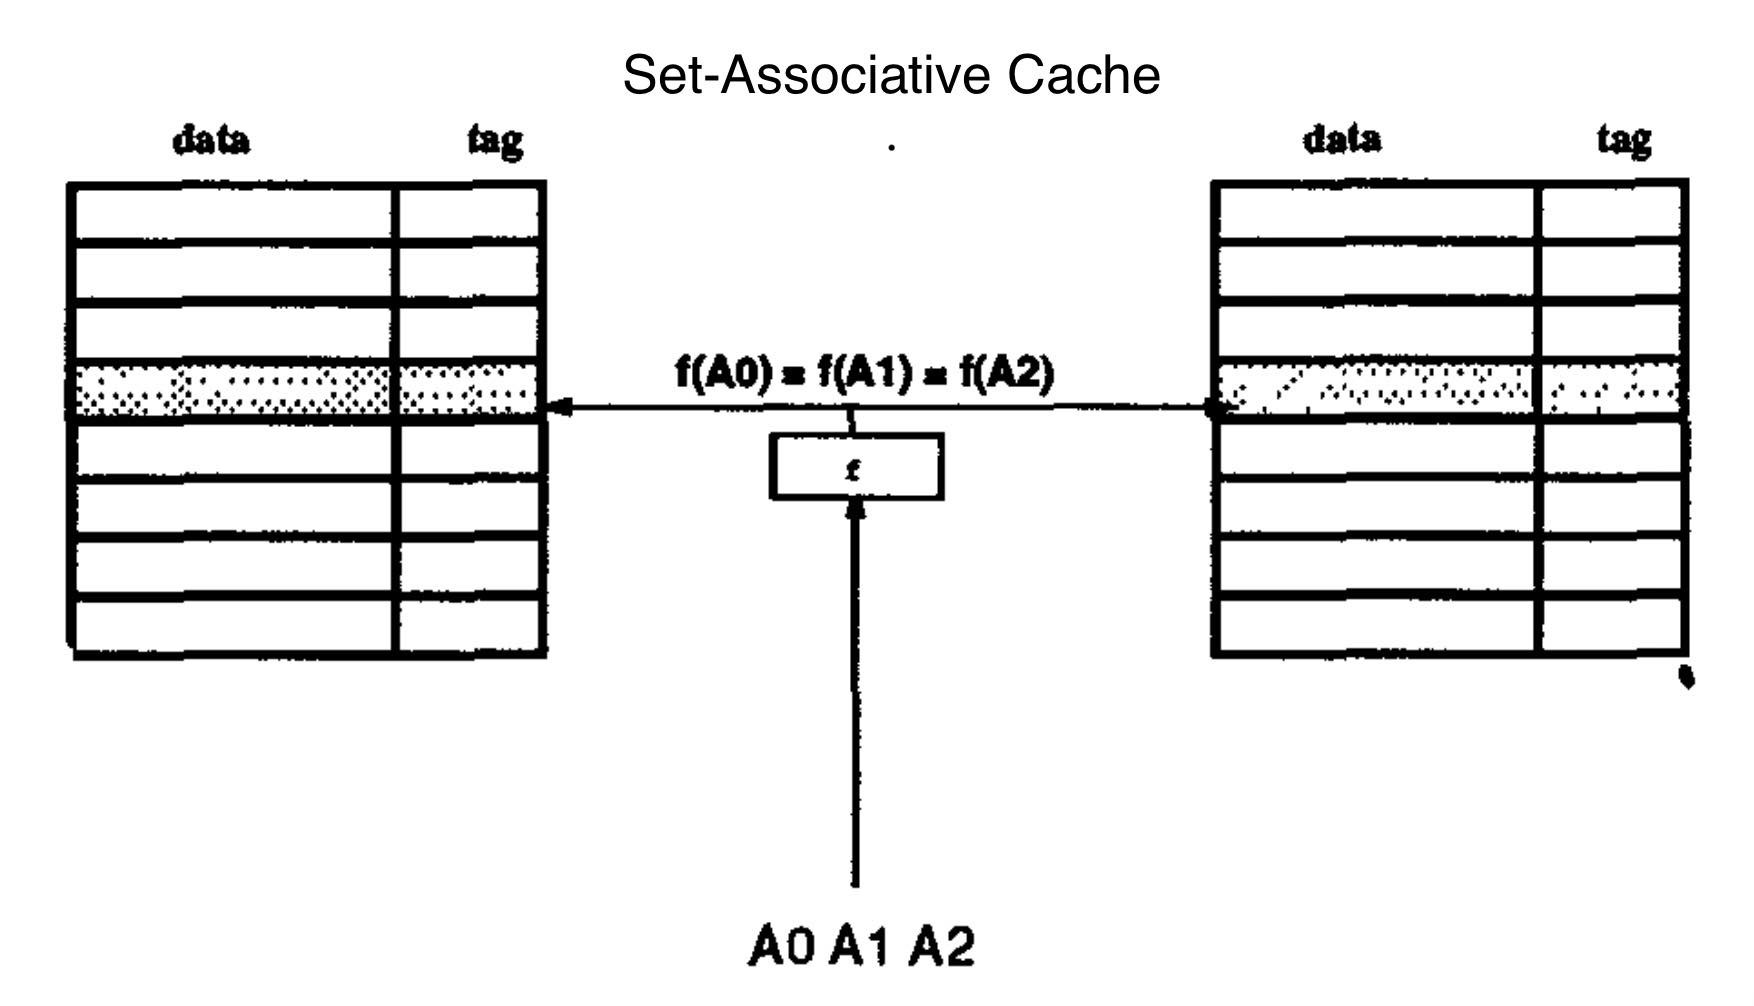
\includegraphics[width=12cm\textwidth,center]{image set associative.jpeg}
    \caption{Set associative cache}
    \label{fig:my_label}
\end{figure}
\\
\begin{figure}
    \centering
    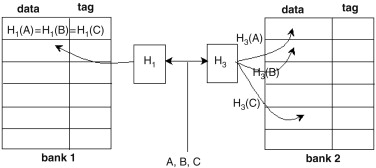
\includegraphics[width=9cm]{image hash.jpg}
    \caption{Skewed associative cache}
    \label{fig:my_label}
\end{figure}

\begin{large}
\subsection{How to choose skewing function}
In this section, we will discuss about the properties that might exhibit functions
chosen for skewing the blocks in the distinct cache banks in order to obtain a good
hit ratio (see [1,3]). We also present the functions which will be used in this
report.\\

\textbf{1 ) Equitability}\\ First of all like in classical caches, for each line
in the cache, the numbers of memory blocks that may be mapped onto this line must be
equal.\\

\textbf{2 ) Inter-bank dispersion}\\ In a usual X-way set-associative cache, when (X+1)
memory blocks contend for the same set in the cache: One of the block must be removed
as there are only X lines available.

\qquad Skewed-associative caches avoid this situation by scattering the data: mapping
functions can be chosen so that whenever two memory blocks conflict for a same line
in bank i, they have a very low probability to conflict for a location in bank j
(Figure 2).\\

\textbf{3 ) Local dispersion in a single bank}\\ Many applications exhibit spatial
locality, therefore the mapping functions must also be chosen so that two "almost"
neighbor memory blocks do not contend for the same physical line in any cache bank.

\qquad The different mapping functions must respect a certain form of local
dispersion on their respective bank; the mapping functions f$_i$ must limit the
number of conflicts when mapping any region of consecutive memory blocks within bank
i.\\

\textbf{4 ) Simple hardware implementation}\\ Mapping functions must have the less
complexity so that it will use a small number of gates and delays.\\

\subsection{How it handles conflict misses}
\textbf{Data dispersion}\\After a single read on a sequence of distinct cache blocks, more blocks are in a skewed-associative cache than on a set-associative cache.\\
\qquad On the other hand, the configuration of data blocks present at the same time in the cache depends on the precise mapping of each data block in the cache. Let us consider a memory block D present in the cache at time t. Among the other possible locations for a block D, there may be a location occupied by an unuseful block (dead block or block which will not be reused for a long time ). Block D may be removed from the cache by a miss. The next time D will be referenced, D can ve mapped in an empty location in bank j, thus increasing the number of useful blocks in the cache. 

\subsection{Replacement policy for skewed-associative caches: a bottleneck}
When a miss occurs in a X-bank caches, the memory block
to be replaced must be chosen among X blocks. Different replacement policies may be used. LRU replacement policy or pseudo-random replacement policy are generally used on set-associative caches.

\qquad LRU replacement policy is generally considered as the most efficient policy. Implementing an LRU policy on a two-way set-associative cache is quite simple. A single bit tag per cache line is sufficient: when a line is accessed, this tag is asserted and the tag of the second line of the set is deasserted.

\qquad Unfortunately, a simple LRU cannot be implemented on a skewed-associative cache. Therefore, some pseudo-LRU replacement policies are used.
\newline\\\\
\textbf{References}\\\\
1)A. Seznec, "A case for two-way skewed associative caches"\\
2)A. Seznec, "Skewed-associative caches"\\
3)F. Bodin, A. Seznec, "Skewed-associativity enhances performance predictability"

\end{large}
\end{document}
